\documentclass[11pt]{article}
\usepackage{graphicx}
\usepackage{subfigure}
    \usepackage{multicol}
\usepackage{multirow}
\usepackage{array, multirow}
\usepackage{hhline}
\usepackage{cprotect} 
\usepackage{tcolorbox}
\usepackage{cite} 
\usepackage{esvect}
\usepackage{amssymb, amsmath, amsbsy}

%    \usepackage[T1]{fontenc}
    % Nicer default font (+ math font) than Computer Modern for most use cases
%    \usepackage{mathpazo}

    % Basic figure setup, for now with no caption control since it's done
    % automatically by Pandoc (which extracts ![](path) syntax from Markdown).
    \usepackage{graphicx}
    % We will generate all images so they have a width \maxwidth. This means
    % that they will get their normal width if they fit onto the page, but
    % are scaled down if they would overflow the margins.
%    \makeatletter
%    \def\maxwidth{\ifdim\Gin@nat@width>\linewidth\linewidth
%    \else\Gin@nat@width\fi}
%    \makeatother
%    \let\Oldincludegraphics\includegraphics
    % Set max figure width to be 80% of text width, for now hardcoded.
%    \renewcommand{\includegraphics}[1]{\Oldincludegraphics[width=.8\maxwidth]{#1}}
    % Ensure that by default, figures have no caption (until we provide a
    % proper Figure object with a Caption API and a way to capture that
    % in the conversion process - todo).
    \usepackage{caption}
    %\DeclareCaptionLabelFormat{nolabel}{}
    %\captionsetup{labelformat=nolabel}
	\usepackage{float}
    \usepackage{adjustbox} % Used to constrain images to a maximum size 
    \usepackage{xcolor} % Allow colors to be defined
    \usepackage{enumerate} % Needed for markdown enumerations to work
    \usepackage{geometry} % Used to adjust the document margins
    \usepackage{amsmath} % Equations
    \usepackage{amssymb} % Equations
    \usepackage{textcomp} % defines textquotesingle
    % Hack from http://tex.stackexchange.com/a/47451/13684:
    \AtBeginDocument{%
        \def\PYZsq{\textquotesingle}% Upright quotes in Pygmentized code
    }
    \usepackage{upquote} % Upright quotes for verbatim code
    \usepackage{eurosym} % defines \euro
    \usepackage[mathletters]{ucs} % Extended unicode (utf-8) support
    \usepackage[utf8x]{inputenc} % Allow utf-8 characters in the tex document
    \usepackage{fancyvrb} % verbatim replacement that allows latex
    \usepackage{grffile} % extends the file name processing of package graphics 
                         % to support a larger range 
    % The hyperref package gives us a pdf with properly built
    % internal navigation ('pdf bookmarks' for the table of contents,
    % internal cross-reference links, web links for URLs, etc.)
    \usepackage{hyperref}
    \usepackage{longtable} % longtable support required by pandoc >1.10
    \usepackage{booktabs}  % table support for pandoc > 1.12.2
    \usepackage[inline]{enumitem} % IRkernel/repr support (it uses the enumerate* environment)
    \usepackage[normalem]{ulem} % ulem is needed to support strikethroughs (\sout)
    
                                % normalem makes italics be italics, not underlines
%Documento
\begin{document}
\begin{equation}
\begin{bmatrix}
\frac{1}{2}+K & -V \\ 
\frac{1}{2}-K & \frac{\mu_2}{\mu_1}V
\end{bmatrix}
\begin{bmatrix}
\varphi_{1d}\\ 
\frac{\partial}{\partial n}\varphi_{1d}
\end{bmatrix}
=\begin{bmatrix}
0\\ 
\frac{\mu_1-\mu_2}{\mu_2}\frac{\partial \varphi_i}{\partial n}
\end{bmatrix}
\end{equation}
Resuelto en 439 iteraciones pero con una velocidad mucho más rápida que la ecuación (2).
\begin{figure}[H]
\centering
\label{fig:Discretizacion BEM y FEM}
\subfigure[Resultado en z=100.]{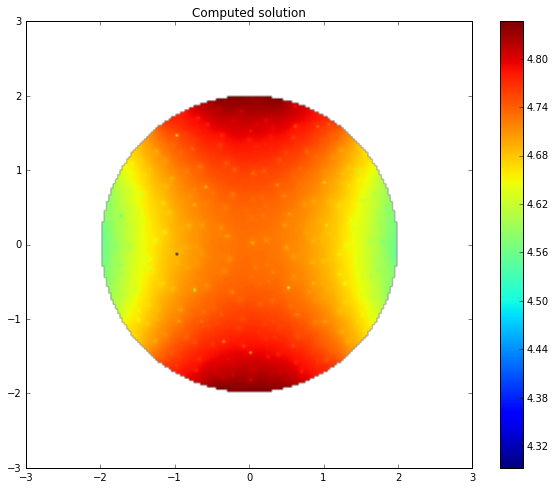
\includegraphics[height=6.4cm]{ecz100.png}}
\subfigure[Resultado en z=90.]{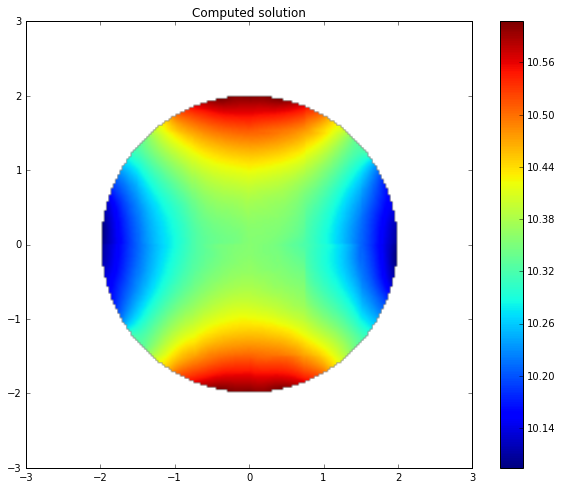
\includegraphics[height=6.4cm]{ecz90.png}}
\subfigure[Resultado en z=50.]{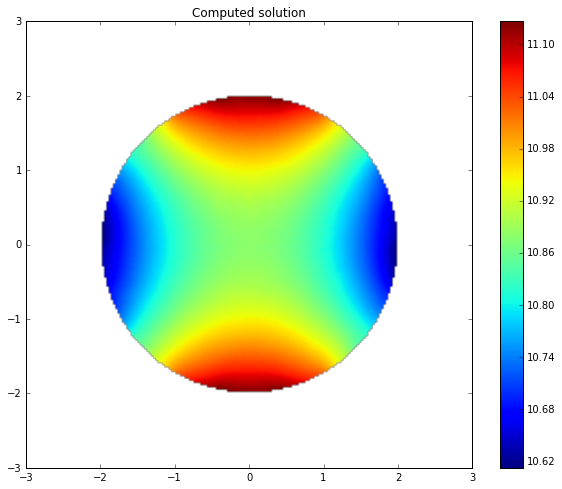
\includegraphics[height=6.4cm]{ecz50.png}}
\subfigure[Resultado en z=0.]{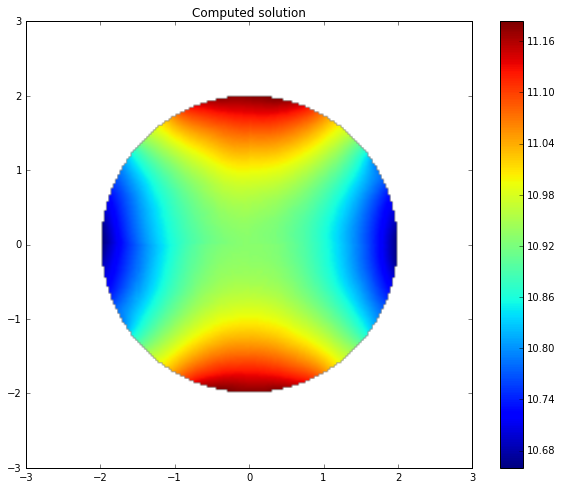
\includegraphics[height=6.4cm]{ec1.png}}
\caption{Resultados en distintas alturas z=0 de la ecuación (1).}
\end{figure}
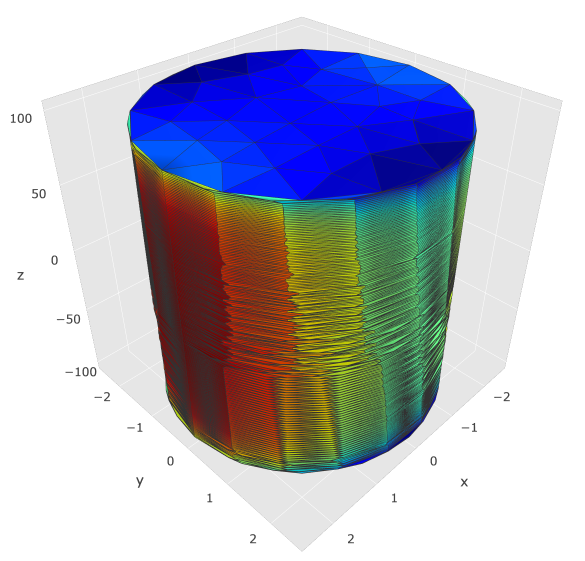
\includegraphics[scale=1.4]{newplot (5).png} \\
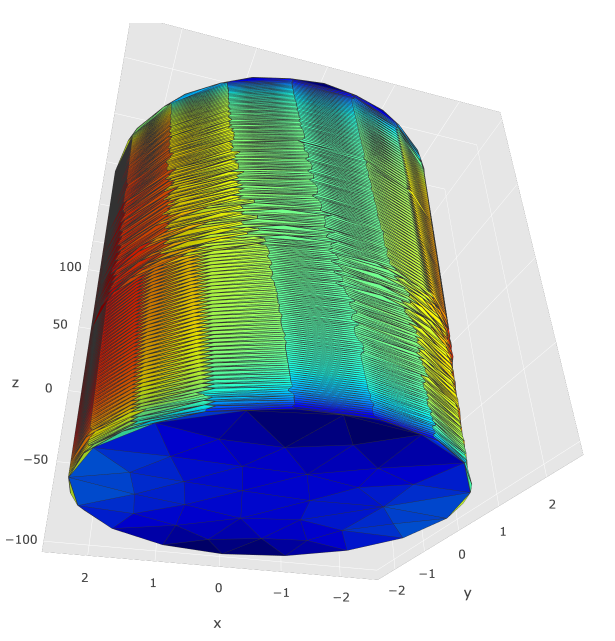
\includegraphics[scale=1.4]{newplot (6).png} 
    
   \newpage 
\begin{equation} 
\begin{bmatrix}
-D_{ext} - D_{int} & \alpha S_{int} + S_{ext}\\
-D'_{ext} - D'_{int} & (\frac{\alpha - 1}{2})+\alpha S'_{int} + S'_{ext}
\end{bmatrix}
\begin{bmatrix}
u^{ext}\\
\frac{\partial u^{ext}}{\partial n}
\end{bmatrix}
=
\begin{bmatrix}
u_{inc}\\
\frac{\partial u_{inc}}{\partial n}
\end{bmatrix}
\label{eq:matriz trans}		 
\end{equation} 
Resuelto en 215 iteraciones para las imagenes en 3D y en 117 para las imagenes en 'Figure 2' (se agrandaron los elementos de la malla, el kernell parecía fallar). Pero el tiempo en resolver estos sistemas era notoriamente mayor.
\begin{figure}[H]
\centering
\label{fig:Discretizacion BEM y FEM}
\subfigure[Resultado en z=100.]{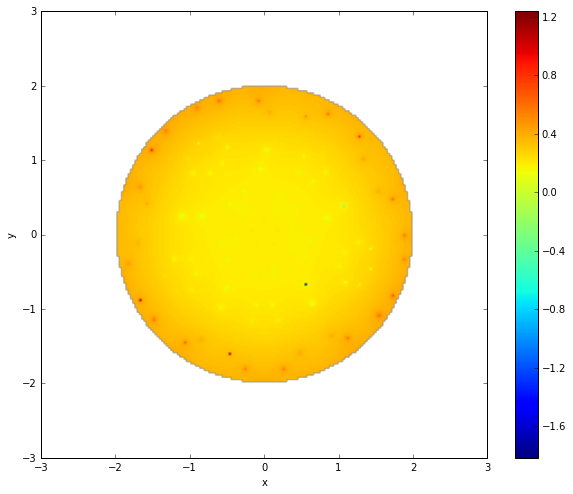
\includegraphics[height=6.4cm]{z=100.png}}
\subfigure[Resultado en z=80.]{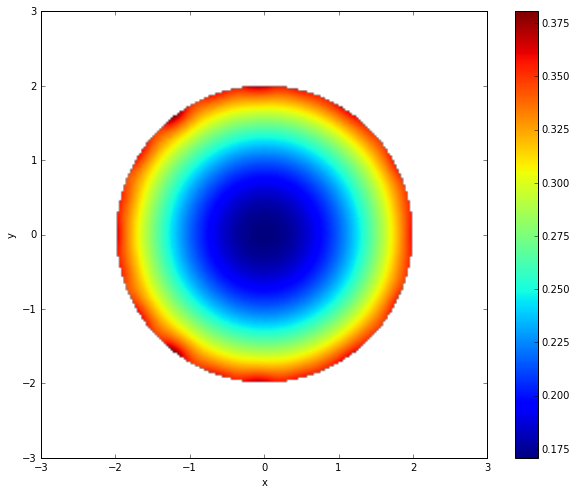
\includegraphics[height=6.4cm]{z=80.png}}
\subfigure[Resultado en z=50.]{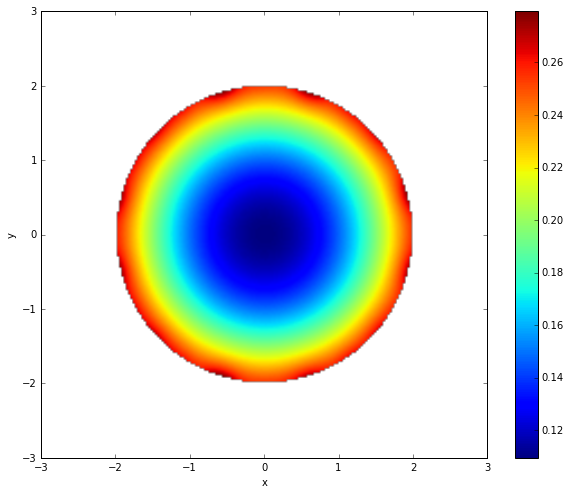
\includegraphics[height=6.4cm]{z=50.png}}
\subfigure[Resultado en z=0.]{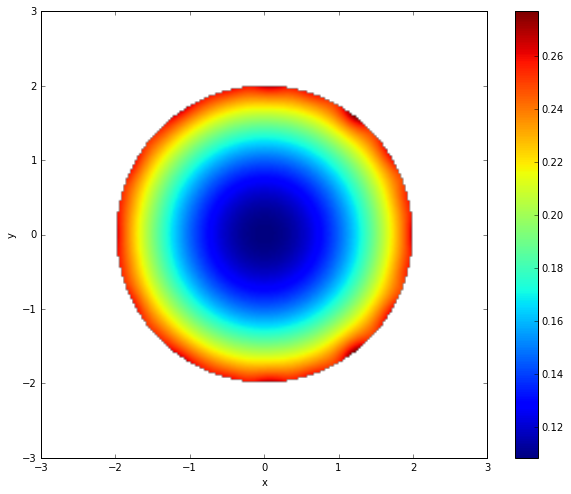
\includegraphics[height=6.4cm]{z=0.png}}
\caption{Resultados en distintas alturas z=0 de la ecuación (2).}
\end{figure}  
\includegraphics[scale=1.4]{newplot (2).png} \\
\includegraphics[scale=1.4]{newplot (3).png} \\
\includegraphics[scale=1.4]{newplot (4).png} 
\end{document}
